\chapter{Realizace}
Po dohodě s vedoucím práce byl zvolen iterační vývoj aplikace. Za účelem postupného vyvíjený částí aplikace, tak aby bylo možné testovat aplikaci na letním semestru 2011/2012. V této kapitole popisuji jednotlivá zadání každé iterace. Jak jsem postupoval k vyřešení zadání a výstupy z jednotlivých iterací. Jednotlivé iterace byly prezentovány na konzultacích s vedoucím práce.

\section{První iterace}
\subsection{Zadání}
První iterace měla za cíl vytvořit základní architekturu aplikace s napojením na KOSapi \cite{kosapi} a k tomu vytvořit funkční část aplikace pro plánování hospitací.

\subsection{Postup}
\subsubsection{Datová vrstva}
Protože aplikace využívá dva datové zdroje KOSapi \ref{kosapi} a databázi aplikace, bylo potřeba nejdřív vyřešit jak se připojit ke KOSapi. V této části vycházím z prototypu aplikace pro správu hospitací. Kde využívá knihovnu z projektu VyVy \cite{vyvy}. Poté bylo potřeba vytvořil modely tak, aby umožnily komunikaci mezi KOSapi a databází aplikace.

\subsubsection{Autentizace a autorizace}
Pro autentizaci, v této fázi vývoje, jsem zatím neimplementoval autentizaci prostřednictvím FElid \ref{felid}. Dočasně jsem pro tento účel použil modul authlogic \cite{authlogic}.

Pro autorizaci používám modul CanCan \cite{cancan}. CanCan je modul pro Ruby on Rails, který určuje, k jakým zdrojům má daný uživatel povolený přístup. Všechna oprávnění jsou definována na jednom místě (třída Ability). Umí filtrovat controllery, views i databázové dotazy.

\subsubsection{Uživatelské prostředí}
Pro vytvoření uživatelského prostředí jsem použil již existující modul Bootstrap \cite{bootstrap} od Twitteru. Použil jsem tuto knihovnu abych si usnadnil implementaci uživatelského prostředí. Knihovna obsahuje kompletní CSS tak i Javascriptové moduly. Mezi další výhody patří licence ta je open-source a další výhodou je známé uživatelské prostředí.

Pro usnadnění implementace Bootstrap \cite{bootstrap} modulu do aplikace jsem využil další dva moduly pro aplikaci. První je modul SimpleForm \cite{simpleform} zjednoduší vytváření formulářů tak, že stačí definovat jedno nadefinovat styl skládání formuláře a v aplikaci už jen jednoduše vytvářet formuláře bez zbytečného stylování. A druhým modulem je WillPaginate \cite{willpaginate}, ten slouží k implementaci stránkování dat.

\subsection{Výstup} 
Výstupem z první iterace vznikla část aplikace, která uměla plánovat hospitace a uměla přímo získávat data z webové služby KOSapi.


\section{Druhá iterace}
\subsection{Zadání}
Zadáním druhé iterace bylo na-implementovat hodnotící formuláře hospitací. Požadavkem bylo možnost upravovat formuláře bez zásahu do kódu aplikace. Dalším cílem bylo potřeba vyřešit problém s KOSapi \ref{kosapi}, který vznikl při přechodu na nový semestr. Stalo se to že služba neudržuje data instancí předmětů z minulých semestrů a tím nebylo možné získat všechny potřebné informace pro starších hospitací.

\subsection{Postup}
\subsubsection{Datová vrstva}
Problém se ztrátou dat jsem vyřešil tak, že  importuji data z KOSapi \ref{kosapi} do databáze aplikace, kterou jsem rozšířil o entity z KOSapi. Pro importování dat bylo potřeba vytvořit rake script, který bude automaticky aktualizovat data.

Jeden ze zádrhelů, který jsem řešil byly \verb|asociace|\footnote{asociace garant, přednášející, vyučující, instruktor a zkoušející.} mezi osobou a instancí předmětu nebo paralelkou. Problém byl v množství asociací mezi entitami. Vyřešil jsem to elegantně za pomocí polymorfních asociací \cite{guide_pa} v Ruby on Rails.

Samotné předělání aplikace nebylo příliš složité stačilo pouze upravit modely tak, aby získávaly data z databáze místo z webové služby. 

\subsubsection{Hodnotící formuláře}
Z důvodu možné změny hodnotících formulářů v budoucnosti. Jsem vytvořil návrh, který umožní vytvářet nové typy formulářů, nebo upravovat již existující. Formuláře se definují šablonou, která definuje základní vlastnosti jako jsou minimální a maximální počet vyplnění, název a kdo může formulář vyplnit. Samotný obsah šablony formuláře se skládá z položek. Položky formuláře mohou být hodnotící tabulka, nadpis, hodnocení, text. Na obrázku \ref{fig:dynamicform} je doménový model dynamický formulářů.

\begin{figure}[h]
\begin{center}
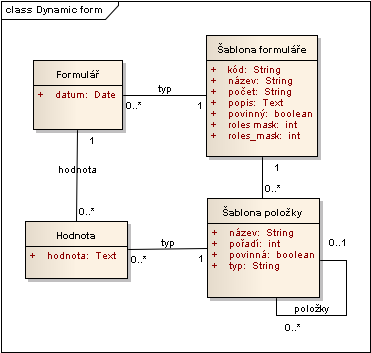
\includegraphics[scale=0.7]{figures/Dynamic_form}
\caption{Doménový model dynamických formulářů}
\label{fig:dynamicform}
\end{center}
\end{figure}

\subsection{Výstup} 
Výstupem této iterace byla aplikace, která již využívala pouze svoji databázi pro zdroj dat a prototyp dynamických formulářů s nadefinovanými hodnotícími formuláři.

%\section{Třetí iterace}
%\subsection{Zadání}
%připravit server pro felid(instalace apache, passenger, rvm, shibboleth), nasazení aplikace, uprava požadavků z konzultací
%sheduled zálohování databáze

%\subsection{Postup}

%\subsection{Výstup} 

